\documentclass[UTF8]{ctexart}

\title{\kaishu 非参数统计}	% 标题
\author{Xifeng Zhang}	% 作者
\date{\heiti \today}	% 日期

\RequirePackage{expl3}

\usepackage{amsmath}
\usepackage[hidelinks]{hyperref}
\usepackage{color}
\usepackage{graphicx}
\usepackage{epstopdf}
\usepackage{caption}
\usepackage{geometry}
\usepackage{booktabs}
\usepackage{listings}
\usepackage{longtable}
\usepackage[dvipsnames]{xcolor}

\lstset{
    language=R, % 设置语言
    basicstyle=\ttfamily, % 设置字体族
    breaklines=true, % 自动换行
    keywordstyle=\bfseries\color{NavyBlue}, % 设置关键字为粗体,颜色为NavyBlue
    morekeywords={}, % 设置更多的关键字,用逗号分隔
    % emph={self}, % 指定强调词,如果有多个,用逗号隔开
    % emphstyle=\bfseries\color{Rhodamine}, % 强调词样式设置
    commentstyle=\itshape\color{black!50!white}, % 设置注释样式,斜体,浅灰色
    stringstyle=\bfseries\color{PineGreen!90!black}, % 设置字符串样式
    columns=flexible,
    % frame=single, % 边框
    % framesep=1em, % 设置代码与边框的距离
    rulecolor=\color[HTML]{fffbf0},
    backgroundcolor=\color[HTML]{fffbf0}
}


\numberwithin{equation}{section}


\newtheorem{thm}{定理}[section]
\newtheorem{definition}{定义}[section]
\newtheorem{chara}{性质}[section]

\newcommand{\diff}{\mathrm{d}}
\newcommand{\tabincell}[2]{\begin{tabular}{@{}#1@{}}#2\end{tabular}}

\geometry{a4paper, scale=0.8}

\begin{document}
\maketitle

\begin{figure}[h]
    \centering
    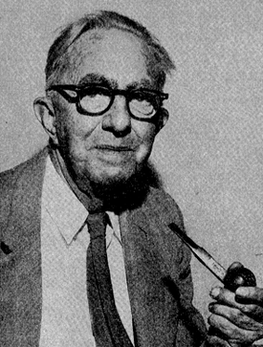
\includegraphics[scale = 0.8]{FrankWilcoxon.png}
    \caption*{Frank Wilcoxon, 1892-1965}
\end{figure}
\thispagestyle{empty}

\clearpage
\tableofcontents

\clearpage
\setcounter{page}{1}

\section{假设检验}
假设检验是统计推断的另一种重要形式,
其任务是通过样本对未知的总体分布特征作出合理的推测,
假设检验可分为参数假设检验和非参数假设检验。

\subsection{显著性检验}
如果一个假设检验问题只提出一个统计假设,
而我们正是为了判断这一统计假设是否成立,
并不同时研究其它统计假设,这类假设检验称为显著性检验

\subsection{假设与检验统计量}
\subsubsection{原假设与备择假设}
原假设又称零假设或基本假设,记为$H_0$;
备择假设又称对立假设或解消假设,记为$H_1$

\subsubsection{双边假设与单边假设}
双边假设一般记为
\begin{equation}
    H_0: \mu = \mu_0 ~~ vs ~~ H_1: \mu \neq \mu_0
    \nonumber
\end{equation}

单边假设一般记为
\begin{equation}
    H_0: \mu \leq(\geq) \mu_0 ~~ vs ~~ H_1: \mu \geq(\leq) \mu_0
    \nonumber
\end{equation}

\subsubsection{检验统计量}
当$H_0$成立时,构造检验统计量,
其分布或渐近分布是已知的,制定一个$H_0$对$H_1$的检验法则

\subsection{拒绝域}
将W记为拒绝域, $\overline{W}$记为接受域
如果根据样本值 $(x_1, x_2, \dots , x_n)$ 求出的检验统计量值$T$,
出现了 $(x_1, x_2, \dots , x_n) \in W$ (小概率事件发生了),
则拒绝$H_0$

\subsection{两类错误}
对假设$H_0$进行检验时,由于样本的随机性,
在进行判断时,无论拒绝$H_0$还是不拒绝$H_0$,都有可能犯两类错误:
第一类错误(又称拒真错误),记为$\alpha$和第二类错误(又称受伪错误),记为$\beta$

在样本量一定的条件下,二者此消彼长,我们通常
会在控制犯第一类错误的条件下,尽量使犯第二类错误小

\subsection{显著性水平}
设样本为x,依据小概率原理,假定$H_0$为真时,有
\begin{equation}
    \alpha = P(\mbox{拒绝}H_0 | H_0 \mbox{为真}) = P(x \in W | H_0 \mbox{为真})
    \nonumber
\end{equation}

其中$\alpha$是预先指定的很小的正数,称为显著性水平(或检验水平)


\subsection{p-value}
拒绝原假设的最小显著性水平
(在原假设成立的条件下,出现样本情况以及更极端的情况发生的概率)

\textcolor{red}{不拒绝原假设不等于接收原假设}

\subsection{假设检验基本方法及其步骤}
\begin{enumerate}
    \item 临界值法
    \begin{itemize}
        \item 给出原假设和备择假设
        \item 构造统计量,计算在原假设下统计量的取值
        \item 给定显著性水平,通过查表得到临界值,得到拒绝域
        \item 比较统计量实现值与临界值,做出拒绝或不拒绝原假设的结论
    \end{itemize}
    
    \item p值法
    \begin{itemize}
        \item 给出原假设和备择假设
        \item 构造统计量,计算在原假设下统计量的取值
        \item 给定显著性水平
        \item 比较判断:$p<\alpha$时,拒绝原假设
    \end{itemize}
\end{enumerate}

\clearpage
\section{非参数统计引言}

\subsection{参数统计方法与非参数统计方法}
\subsubsection{参数统计方法}
参数统计中提出问题时,产生数据的总体的分布形式或分布族往往是
给定的或者是假定了的,所不知道的仅仅是一些参数的值或他们的范围。
参数统计的研究任务就是对这些未知的参数进行统计推断,
如:点估计、区间估计和假设检验等。

\subsubsection{非参数统计方法的局限性}
参数统计在实际运用时有其不可避免的局限性:
\begin{enumerate}
    \item 有时关于总体分布形式假定缺乏充分根据
    \item 样本可能并非来自具有假定分布的总体
    \item 样本数据可能存在系统误差,即:数据根本不是来自一个总体,或者数据因为种种原因被严重污染
\end{enumerate}

在这三种情况下,在假定总体分布的情况下进行推断的做法就可能产生错误的结论。
于是,人们希望在不假定总体分布的情况下,尽量从数据本身来获得所需要的信息。
这就是非参数统计的宗旨。 

\subsubsection{非参数统计方法}
非参数统计方法就是在对总体分布形式无假定,
或仅作一些诸如对称性、连续性之类的非常一般性假设条件而进行推断的统计方法。

\subsubsection{非参数统计的特点}
\begin{enumerate}
    \item 应用广泛:对总体假定较少,所以总体分布形式对其影响小,有广泛的适用性,结果的稳定性较好。
    \item 通常效率较低:非参数统计是通用工具,而参数统计是专用工具
\end{enumerate}

\subsubsection{参数统计方法和非参数统计方法的比较}
\begin{itemize}
    \item 参数统计问题总体分布的形式是已知的,仅含有有限个未知的参数,
    在总体分布已知时使用参数方法能够充分利用总体分布已知这一信息,
    使得统计分析更有效。
    \item 非参数统计问题不满足 “总体分布的形式是已知的, 仅含有有限个未知的参数”,
    有相当好的稳健性,计算简单.处理问题广泛,
    在多数分布未知的情况下非参数方法更有效。
\end{itemize}

\subsection{连续性修正}
实践中,为处理问题方便,常用连续型分布去近似离散型分布,
设X为离散型随机变量,Y为连续型随机变量,$E(X)=E(Y)$, $Var(X)=Var(Y)$,
对$x$加或者减部分邻域范围的调整就称为连续性修正

\begin{equation}
    P(X \leq x) \approx P(Y \leq x + \dfrac{1}{2})
\end{equation}

\begin{equation}
    P(X \geq x) \approx P(Y \geq x - \dfrac{1}{2})
\end{equation}

\begin{equation}
    P(X = x) \approx P(x - \dfrac{1}{2} \leq Y \leq x + \dfrac{1}{2})
\end{equation}

\subsection{顺序统计量}
设样本 $(X_1, X_2,\dots, X_n)$ 为简单随机样本,
将其按由小到大顺序排列为$X_{(1)}, X_{(2)}, \dots, X_{(n)}$,
称为样本的顺序统计量,其中$X_{(i)}$为第i个顺序统计量,
$X_{(1)}$为最小顺序统计量,$X_{(n)}$为最大顺序统计量。

由此可得
样本极差定义为 $W = X_{(n)} - X_{(1)}$,
样本中列数定义为$\dfrac{X_{(1)}+X_{(n)}}{2}$,
样本均值定义为 $\overline{X} = \sum_{i=1}^{n} \dfrac{X_{(i)}}{n}$.

\subsubsection{顺序统计量的分布}
设样本 $(X_1, X_2,\dots, X_n)$为来自总体的i.d.d样本,

\subsubsection{$X_{(r)}$的分布}

\begin{equation}
    \begin{split}
        F_r(x) 
        & = P(X_{(r)} \leq x) = P(\mbox{至少} r \mbox{个} X_i \mbox{小于或等于} x) \\
        & = \sum_{i=r}^{n} \tbinom{n}{r} F^i(x) [1-F(x)]^{n-i}
    \end{split}
\end{equation}

\begin{equation}
    f_r(x) = \dfrac{n!}{(r-1)!(n-r)!} F^{r-1}(x) f(x) [1 - F(x)]^{n-r}
\end{equation}

\subsubsection{$X_{(r)}$和$X_{(s)}$的联合分布}

\begin{equation}
    f_{r,s}(x,y) = 
    \begin{cases}
        C(n,r,s) F^{r-1}(x)f(x)[F(y)-F(x)]^{s-r-1}f(y)[1-F(y)]^{n-s} &, x<y \\
        0 &,x \geq y
    \end{cases}
\end{equation}

其中$C(n,r,s) = \dfrac{n!}{(r-1)!(s-r-1)!(n-s)!}$

\subsection{分位数}
数据中有$\pi \times \%$小于或等于此数,
$(1 - \pi) \times 100 \%$大于或等于此数的数值。
如果有n个数据,那么$Q_{\pi}$就是n个样本中的第$[n \pi]$位或$[n \pi]+1$位数值,
即当$[n \pi]$为整数时,取$[n \pi]$,
当$[n \pi]$不是整数时,取大于$[n \pi]$的最小整数。
四分位点有三个:25$\%$分位数(下四分位点),50$\%$分位数(中位数),
75$\%$分位数(上四分位点)。

其中,中位数可由顺序统计量表示为:
\begin{equation}
    M_e = 
    \begin{cases}
        X_{(\frac{n+1}{2})} &, if~n~is~an~odd~number \\
        \dfrac{X_{(\frac{n}{2})}+X_{(\frac{n}{2}+1)}}{2} &, if~n~is~an~even~number
    \end{cases}
\end{equation}

\subsection{修整均值(切尾均值)}
一般样本均值受极端值的影响大,为了比较合理地反映总体平均分布状态,
定义修整均值为
\begin{equation}
    T_{(j)} = \sum_{i=j+1}^{n-j} \dfrac{X_{(i)}}{n-2j}
\end{equation}

\subsubsection{修整均值与均值}
\begin{equation}
    T_{(0)} = \overline{X}
\end{equation}

\subsubsection{修整均值与中位数}

n为奇数时
\begin{equation}
    T_{(\frac{n}{2}-1)} = M_e
\end{equation}

n为偶数时
\begin{equation}
    T_{(\frac{n-1}{2})} = M_e
\end{equation}

\subsection{层与层数}
首先对数据由小到大进行排序,并定义层(depth)数为:

\begin{equation}
    d = 
    \begin{cases}
        \dfrac{n}{2} &, n \mbox{偶数} \\[1em]
        \dfrac{n+1}{2} &, n \mbox{奇数}
    \end{cases}
\end{equation}

可以得到:
\begin{enumerate}
    \item 最大、最小值的层数为:$d(X_{(n)}) = d(X_{(1)})=1$

    \item 上下四分位数所在层数为:
    \begin{equation}
        d(Q) = d(Q_U) = d(Q_L) = 
        \begin{cases}
            \dfrac{n+3}{4} & ,n \mbox{为奇数} \\[1em]
            \dfrac{n+2}{4} & ,n \mbox{为偶数}
        \end{cases}
    \end{equation}
    
    \item 中位数所在层数为:
    \begin{equation}
        d(M_e) = 
        \begin{cases}
            \dfrac{n+1}{2} & ,n \mbox{为奇数} \\[1em]
            \dfrac{n}{2} & ,n \mbox{为偶数}
        \end{cases}
    \end{equation}
\end{enumerate}

\subsection{秩与秩统计量}
\subsubsection{定义}
\begin{definition}
    设样本 $(X_1, X_2,\dots, X_n)$ 为简单随机样本, 
    记$(X_1, X_2,\dots, X_n)$ 中不超过$X_i$的数据的个数为$X_i$的秩,
    记为$R_i = rank(X_i)$,$X_i$为第$R_i$个顺序统计量,
    此处
    \begin{equation}
        R_i = \sum_{j}^{n} I(X_j \leq X_i)
    \end{equation}
\end{definition}

\begin{definition}
    令$R = (R_1, R_2, \dots, R_n)$,
    R是由样本产生的统计量,
    它是$\left\{ 1,2,\dots,n \right\}$的一个排列,
    称R及基于R派生的一些统计量为秩统计量.
\end{definition}

\subsubsection{不打结样本与有结数据}
当数据中有重复数据时,称数据中存在“结”(tie)。
设样本 $(X_1, X_2,\dots, X_n)$ 为简单随机样本, 
将数据排序后,相同的数据点组成一个“结”,称重复数据的个数为
\textcolor{red}{结长},
结长为1的称为\textcolor{red}{平凡结}

对于有结数据的秩作如下定义:
\begin{definition}
    将样本$(X_1, X_2,\dots, X_n)$按照从小到大排序后,记结果如下:
    \begin{equation}
        \begin{split}
            X_{(1)} 
            & = \dots = X_{(\tau_1)} < X_{(\tau_1+1)} = 
            \dots = X_{(\tau_1+\tau_2)} < \dots < \\
            & X_{(\tau_1+\dots+\tau_{g-1}+1)} = \dots 
            = X_{(\tau_1+\dots+\tau_{g})}
        \end{split}
        \nonumber
    \end{equation}

    其中,g是样本中结的个数,
    $\tau_i$是第i个结的长度,
    $(\tau_1,\dots,\tau_g)$是g个正整数,
    $\sum_{i=1}^g \tau_i = n$,称$(\tau_1,\dots,\tau_g)$为结统计量。
\end{definition}
\begin{definition}
    对于第i组样本的秩都是相同的,是第i组样本原秩的平均:
    \begin{equation}
        \begin{split}
            r_i 
            & = \dfrac{1}{\tau_i} \sum_{k=1}^{\tau_i} (\tau_1 + \dots + \tau_{i-1} + k) \\
            & = \tau_1 + \dots + \tau_{i-1} + \dfrac{1+\tau_i}{2}
        \end{split}
    \end{equation}
\end{definition}

\subsubsection{秩统计量的性质}
设$(X_1, X_2,\dots, X_n)$是来自具有连续分布的$F(x)$的i.i.d样本,
$R = (R_1, R_2, \dots, R_n)$是$\left\{ 1,2,3,\dots,n\right\}$的一个排列,
则对$\left\{ 1,2,3,\dots,n\right\}$的任一排列$\left\{i_1,i_2,i_3,\dots,i_n\right\}$, 
$R = (R_1, R_2, \dots, R_n)$的联合分布为
\begin{equation}
    P[R=(i_1,i_2,\dots,i_n)]=\dfrac{1}{n!}
\end{equation}
注意到
\begin{itemize}
    \item 对于独立同分样本来说,秩的分布与总体分布无关
    \item R在$\left\{ 1,2,3,\dots,n\right\}$的全体排列(共n!个)构成空间上服从离散均匀分布
\end{itemize}
对于R的任一边缘分布亦均为离散均匀分布:
\begin{equation}
    P(R_i = r) = \dfrac{1}{n} ~ (i=1,2,\dots,n)
\end{equation}
\begin{equation}
    P(R_i = r, R_j = s) = \dfrac{1}{n(n-1)} ~ (r,s=1,2,\dots,n;i \neq j,r \neq s)
\end{equation}
因此可以导出边缘分布的期望、方差以及协方差:
\begin{equation}
    \begin{matrix}
        E(R_i) = \dfrac{n+1}{2} \\[1em]
        Var(R_i) = \dfrac{(n+1)(n-1)}{12} \\[1em]
        Cov(R_i, R_j) = -\dfrac{n+1}{12}
    \end{matrix}
    \nonumber
\end{equation}
这说明,虽然$X_1,\dots,X_n$独立同分布,但$R_1,\dots,R_n$同分布相关不独立


\subsection{线性秩统计量}
\subsubsection{线性符号秩统计量}
除了需要考虑顺序,有时需考虑数量本身的关系,因此引入线性秩统计量:
\begin{definition}
    设$R_i^+$为$|X_i|$在$|X_1|,|X_2|,|X_3|,\dots,|X_n|$中的秩,
    $a_n^+ (·)$为定义在整数$1,2,\dots,n$上的非降函数,
    即满足$0 \leq a_n^+ (1) \leq \dots \leq a_n^+ (n),a_n^+ (n)>0$
    则称$S_n^+$为线性符号秩统计量
    \begin{equation}
        S_n^+ = \sum_{i=1}^n a_n^+ (R_i^+) I(X_i>0)
    \end{equation}
\end{definition}

若$a_n^+ (i) = 1$,得到符号统计量(观察值中正数的个数)
\begin{equation}
    S^+ = \sum_{i=1}^n a_n^+ (R_i^+) I(X_i>0) = \sum_{i=1}^n I(X_i>0)
\end{equation}

若$a_n^+ (i) = i$,得到Wilcoxon符号秩统计量(观察值中正数对应的$R_i^+$的和)
\begin{equation}
    W^+ = \sum_{i=1}^n a_n^+ (R_i^+) I(X_i>0) = \sum_{i=1}^n R_i^+ I(X_i>0)
\end{equation}

设$(X_1,\dots,X_n)$为来自以0为对称中心的连续分布的总体的独立同分布的样本,则
\begin{equation}
    \begin{matrix}
        E(S_n^+) = \dfrac{1}{2} \sum_{i=1}^n a_n^+ (i) \\[1em]
        Var(S_n^+) = \dfrac{1}{4}\sum_{i=1}^n [a_n^+ (i)]^2
    \end{matrix}
    \nonumber
\end{equation}

\subsubsection{线性秩统计量}
\begin{definition}
    设$(X_1,\dots,X_n)$为样本,秩为$R=(R_1,\dots,R_n)$,
    $a_n^+ (·)$(称为记分函数,简称记分)
    和$c_n(i)$(称为回归常数)为定义在整数$1,2,\dots,n$上的函数,
    则称$S_n$为线性秩统计量
    \begin{equation}
        S_n = \sum_{i=1}^n c_n(i) a_n (R_i) I(X_i>0)
    \end{equation}
\end{definition}

若$(X_1,\dots,X_n)$为i.d.d连续分布,
即$(R_1,\dots,R_n)$在$1,2,\dots,n$上有均匀分布,
这时线性秩统计量的期望和方差为:
\begin{equation}
    \begin{matrix}
        E(s_n) = n \overline{a} \overline{c} \\[1em]
        Var(S_n)= \dfrac{1}{n-1} \sum_{i=1}^n (c_n (i) - \overline{c})^2 \sum_{i=1}^n (a_n (i) - \overline{a})^2
    \end{matrix}
    \nonumber
\end{equation}
式中,$\overline{a} = \dfrac{1}{n}\sum_{i=1}^n a_n(i)$,$\overline{c} = \dfrac{1}{n}\sum_{i=1}^n c_n(i)$

\clearpage
\section{单样本问题}
\subsection{广义符号检验}
\subsubsection{总体中位数}
\begin{definition}
    设X是一个随机变量,$M(or~M_e)$是一个常数,满足:
    \begin{equation}
        P(X \leq M) \geq \dfrac{1}{2},P(X \geq M) \geq \dfrac{1}{2}
        \nonumber
    \end{equation}
    则称M为(总体)中位数
\end{definition}

\begin{itemize}
    \item 总体中位数必定存在
    \item 总体中位数未必唯一
    \item 对于连续分布,使得$F(M)=\int_{-\infty}^M f(x) \,dx = \dfrac{1}{2}$的M即是一个总体中位数
    \item 对于对称分布,中位数就是分布中心——位置中心
\end{itemize}

\subsubsection{总体$\pi$分位数}
\begin{definition}
    设X是一个随机变量,$Q_{\pi}$是一个常数,满足:
    \begin{equation}
        P(X \leq Q_{\pi}) \geq \pi,P(X \geq Q_{\pi}) \geq 1-\pi
        \nonumber
    \end{equation}
    则称$Q_{\pi}$为(总体)$\pi$分位数
\end{definition}

\subsubsection{符号统计量}
\begin{equation}
    \begin{cases}
        S^+ = \sum_{i=1}^{n} I(X_i > q_0) = \sum_{i=1}^{n} I(X_i - q_0 > 0) \sim B(n, 1-\pi) \\[1em]
        S^- = \sum_{i=1}^{n} I(X_i < q_0) = \sum_{i=1}^{n} I(X_i - q_0 < 0) \sim B(n, \pi)
    \end{cases}
\end{equation}

\begin{itemize}
    \item $S^+$表示大于$q_0$的个数,即正号的个数
    \item $S^-$表示小于$q_0$的个数,即负号的个数
\end{itemize}

\subsubsection{$\pi$分位数检验}

\begin{center}
    \begin{longtable}{cccc}
        \caption{$\pi$分位数检验} \\ \toprule
        \endfirsthead
        \multicolumn{3}{l}{(续上页)} \\ \toprule
        \endhead
        \bottomrule
        \multicolumn{3}{l}{(接下页)} \\[2ex]
        \endfoot
        \bottomrule
        \endlastfoot
        检验类型 & 右侧检验 & 左侧检验 & 双侧检验 \\
        \hline
        原假设$H_0$ & $Q_{\pi} = q_0$ & $Q_{\pi} = q_0$ & $Q_{\pi} = q_0$ \\
        备择假设$H_1$ & $Q_{\pi} > q_0$ & $Q_{\pi} < q_0$ & $Q_{\pi} \neq q_0$ \\
        检验统计量 & $S^-(or~S^+)$ & $S^-(or~S^+)$ & $S^-(or~S^+)$ \\
        $H_0$为真时$\frac{S^-}{n}$ & 应在$\pi$附近 & 应在$\pi$附近 & 应在$\pi$附近 \\
        $H_0$为真时$\frac{S^+}{n}$ & 应在$1-\pi$附近 & 应在$1-\pi$附近 & 应在$1-\pi$附近 \\
        $H_1$为真时$\frac{S^-}{n}$ & 比$\pi$偏小 & 比$\pi$偏大 & 比$\pi$偏小(偏大)\\
        $H_1$为真时$\frac{S^+}{n}$ & 比$1-\pi$偏大 & 比$1-\pi$偏小 & 比$1-\pi$偏大(偏小)\\
        p值($K=S^-$) & $P_{H_0}(K \leq s^-)$ & $1-P_{H_0}(K \leq s^- -1)$ & $2\min \left\{ {P_{H_0}(K \leq s^-), P_{H_0}(K \geq s^-)} \right\}$ \\
        p值($K=S^+$) & $1-P_{H_0}(K \leq s^+ - 1)$ & $P_{H_0}(K \leq s^+)$ & $2\min \left\{ {P_{H_0}(K \geq s^+), P_{H_0}(K \leq s^+)} \right\}$
    \end{longtable}
\end{center}

\subsubsection{中位数检验}

\begin{center}
    \begin{longtable}{cccc}
        \caption{中位数检验} \\ \toprule
        \endfirsthead
        \multicolumn{3}{l}{(续上页)} \\ \toprule
        \endhead
        \bottomrule
        \multicolumn{3}{l}{(接下页)} \\[2ex]
        \endfoot
        \bottomrule
        \endlastfoot
        检验类型 & 右侧检验 & 左侧检验 & 双侧检验 \\
        \hline
        原假设$H_0$ & $M_e = M_0$ & $M_e = M_0$ & $M_e = M_0$ \\
        备择假设$H_1$ & $M_e > M_0$ & $M_e < M_0$ & $M_e \neq M_0$ \\
        检验统计量 & $K = min\left\{ S^{+},S^{-} \right\}$ & $K = min\left\{ S^{+},S^{-} \right\}$ & $K = min\left\{ S^{+},S^{-} \right\}$ \\
        统计量实现值 & $k = min\left\{ s^{+},s^{-} \right\}$ & $k = min\left\{ s^{+},s^{-} \right\}$ & $k = min\left\{ s^{+},s^{-} \right\}$ \\
        p值 & $P(K \leq k)$ & $P(K \leq k)$ & $2P(K \leq k)$
    \end{longtable}
\end{center}

\subsubsection{大样本正态近似}
n比较小时,可用二项分布的公式计算精确概率,
但当n较大时,精确计算概率太麻烦,所以在大样本时可以做近似计算

\begin{center}
    \begin{longtable}{ccc}
        \caption{大样本正态近似} \\ \toprule
        \endfirsthead
        \multicolumn{3}{l}{(续上页)} \\ \toprule
        \endhead
        \bottomrule
        \multicolumn{3}{l}{(接下页)} \\[2ex]
        \endfoot
        \bottomrule
        \endlastfoot
            & 分位数检验 & 中位数检验 \\
        \midrule
        二项分布统计量 & $K(=S^{-}) \sim B(n, \pi)$ & $K \sim B(n, 0.5)$ \\[1em]
        大样本正态近似 & $Z = \dfrac{K - E(K)}{\sqrt{Var(K)}} \sim N(0, 1)$ & $Z = \dfrac{K - \frac{n}{2}}{\sqrt{\frac{n}{4}}} \sim N(0, 1)$ \\[2em]
        连续性修正统计量 & $Z = \dfrac{K \pm 0.5 - E(K)}{\sqrt{Var(K)}} \sim N(0, 1)$ & $Z = \dfrac{K + 0.5 - \frac{n}{2}}{\sqrt{\frac{n}{4}}} \sim N(0, 1)$
    \end{longtable}
\end{center}

这里做了连续性修正,但是有时,用不用连续性修正,对结果影响不大。

\subsubsection{R语言实现}

检验大城市的花销指数(ExpensiveCities.txt)的下四分位数是否为64
\begin{center}
    \begin{lstlisting}
        # Import Data ExpensiveCities.txt
        x <- read.table("D:/R/TEST/Non_parameter_data/ExpensiveCities.txt")
        summary(x)
    \end{lstlisting}
\end{center}
样本下四分位数为50.85,作出假设为:
\begin{equation}
    H_0:Q_{\pi} = 64 ~ VS ~ H_1: Q_{\pi} < 64
    \nonumber
\end{equation}
使用直接计算p值的方法
\begin{center}
    \begin{lstlisting}
        # p-value
        p <- 1 - pbinom(sum(x<64)-1, dim(x)[1], 0.25)
    \end{lstlisting}
\end{center}
使用R的程序包binom.test
\begin{center}
    \begin{lstlisting}
        # binom.test
        ?binom.test
        binom.test(sum(x<64), dim(x)[1], 0.25, alternative="greater")
    \end{lstlisting}
\end{center}
自定义函数进行检验
\begin{center}
    \begin{lstlisting}
        # sign.test.R
        one.sample.sign.test <- function(x, p, q0) {
            s1 <- sum(x < q0)
            s2 <- sum(x > q0)
            n <- s1 + s2
            p1 <- pbinom(s1, n, p)
            p2 <- 1 - pbinom(s1 - 1, n, p)
            if (p1 > p2) {
                m1 <- "One tail test:H1:Q<q0"
            } else {
                m1 <- "One tail test: H1: Q>q0"
            }
            p.value <- min(p1, p2)
            m2 <- "Two tails test"
            p.value2 <- 2 * p.value
            if (q0 == median(c(t(x)))) {
                p.value <- 0.5
                p.value2 <- 1
            }

            list(
                Sign.test1 = m1, p.values.of.one.tail.test = p.value,
                p.value.of.two.tai.test = p.value2
            )
        }
        one.sample.sign.test(x, 0.25, 64)

        source("D:/R/TEST/000 R files/nonparatest.R")
    \end{lstlisting}
\end{center}

\subsection{基于符号检验的中位数和分位点置信区间}
\subsubsection{中位数的置信区间}
\begin{definition}
    对于显著性水平$\alpha$的中位数的双边检验:$H_0:M_e = M_0~vs.~H_1:M_e \neq M_0$
    存在不会使$H_0$被拒绝的那些原假设点$M_0$的集合
    \begin{equation}
        X_{(1)} \leq X_{(2)} \leq \dots \leq X_{(i)} \leq \dots \leq M_e \leq \dots \leq X_{(j)} \leq \dots \leq X_{(n)}
        \nonumber
    \end{equation}
    找到合适的i和j,使得 $P \left\{ X_{(i)} < M_e < X_{(j)} \right\} \geq 1 - \alpha$,则 $(X_{(i)}, X_{(j)})$ 是 $M_e$ 的一个置信度为 $100(1 - \alpha) \%$ 的置信区间
\end{definition}

对$(X_{(i)} ,X_{(j)})$而言,前面有$i$个观察值,后面有$n-j+1$个
观察值,$i \neq n-j+1$时,区间$(X_{(i)} ,X_{(j)})$关于 $M_e$ 非对称。

\subsubsection{中位数的对称置信区间}
考虑对称区间
\begin{equation}
    (X_{(k)} ,X_{(n-k+1)}),k = 1,2,\dots 
    \begin{cases}
        \dfrac{n}{2} &, n \mbox{为偶数} \\[1em]
        \dfrac{n-1}{2} &, n \mbox{为奇数}
    \end{cases}
    \nonumber
\end{equation}

不失一般性,假定$S^{-} < S^{+}$,如果在$S^- = k-1$时可以拒绝原假设,
在$S^- > k-1$时不能拒绝原假设
(也就是说$S^- = k-1$是最大的能够拒绝原假设的$S^-$的数目)
则原假设在开区间$(X_{(k)} ,X_{(n-k+1)})$之外时会被拒绝。

\begin{equation}
    \begin{split}
        P(X_{(k)} < M_e < X_{(n-k+1)}) 
        & = 1 - P(S^- \leq k-1) - P(S^- \geq n-k+1) \\
        & = 1 - 2P(S^- \leq k-1)
    \end{split}
    \nonumber
\end{equation}

\subsubsection{中位数的大样本正态近似置信区间}
$K \sim B(n,0.5)$,
样本量充分大时,有$Z = \dfrac{K + 0.5 - E(K)}{\sqrt{Var(K)}} \sim N(0, 1)$

\begin{equation}
    P(Z \leq |Z_{\frac{\alpha}{2}}|) = 1 - \alpha
\end{equation}
整理得
\begin{equation}
    P(\dfrac{n}{2} - 0.5 - Z_{\frac{\alpha}{2}} \dfrac{\sqrt{n}}{2} \leq K \leq \dfrac{n}{2} - 0.5 + Z_{\frac{\alpha}{2}} \dfrac{\sqrt{n}}{2}) = 1 - \alpha
\end{equation}
进一步解得
\begin{equation}
    k = [\dfrac{n}{2} - 0.5 - Z_{\frac{\alpha}{2}}]
\end{equation}
其中$[·]$为取整

\subsubsection{R语言实现}

随机抽取的22个企业的纳税额数据(tax.txt)
\begin{center}
    \begin{lstlisting}
        # Import Data tax.txt
        tax <- read.table("D:/R/TEST/002 data/003_Non_parameter_data/tax.txt")
        summary(tax)
        x <- tax$V1
    \end{lstlisting}
\end{center}

\begin{center}
    \begin{lstlisting}
        # Median confidence interval
        mci <- function(x, alpha=0.05){
            # Median confidence interval 1
            x <- sort(x)
            n <- length(x);b <- 0;i <- 0
            while(b <= alpha/2 & i <= floor(n/2)){
            b <- pbinom(i, n, 0.5);
            k1 <- i;
            k2 <- n - i + 1;
            a <- 2 * pbinom(k1-1, n, 0.5);
            i <- i + 1
            }
            z <- c(k1, k2, a, 1-a);
            z2 <- "Entire range!"
            
            if (k1 >= 1) {
            out <- list(Confidence.level=1-a, CI=c(x[k1], x[k2]))
            } else {
            out <- list(Confidence.level = 1-2*pbinom(0, n, 0.5), CI = z2)
            }
            out
        }
        
        mci2 <- function(x, alpha=0){
            # Median confidence interval 2
            x <- sort(x)
            n <- length(x);q <- 0.5
            m <- floor(n*q);
            s1 <- pbinom(0:m, n, q)
            s2 <- pbinom(m:(n-1), n, q, low = F)
            ss <- c(s1, s2);nn <- length(ss)
            a <- NULL;
            for (i in 0:m) {
            b1 <- ss[i+1];
            b2 <- ss[nn-i];
            b <-  b1 + b2;
            d <- 1 - b;
            if((b)>1) break
            a = rbind(a, c(b, d, x[i+1], x[n-i]))
            }
            colnames(a) <- c("p-value", "Confidence level", 
                            "lower limit", "Higher limit")
            if (a[1, 1] > alpha) {
            out <- a
            } else {
            for (i in 1:nrow(a)) {
                if (a[i, 1] > alpha) {
                out <- list(a[i-1, 1], a[i-1, 2], a[i-1, 3:4]);
                break
                }
            }
            }
            out
        }
        
        source("D:/R/TEST/000 R files/nonparatest.R")
        MCI <- mci(x, 0.05)
        MCI.all <- mci2(x)
    \end{lstlisting}
\end{center}

\begin{center}
    \begin{lstlisting}
        # Quantile confidence interval
        qci <- function(x, alpha=0.05, q=0.25){
            # Quantile confidence interval
            x <- sort(x);
            n <- length(x);
            a <- alpha/2;
            r <- qbinom(a, n, q);
            s <- qbinom(1-a, n, q);
            CL <- pbinom(s, n ,q) - pbinom(r-1, n, q)
            
            if (r == 0) {
            lo <- NA 
            } else {
            lo <- x[r]
            }
            
            if (s == n) {
            up <- NA 
            } else {
            up <- x[s+1]
            }
            
            list(c("lower limit"=lo, "upper limit"=up),
                "1-alpha"=1-alpha, "true confidence level"=CL)
        }

        source("D:/R/TEST/000 R files/nonparatest.R")
        QCI <- qci(x)
    \end{lstlisting}
\end{center}

\subsection{Wilcoxon符号秩检验}

\subsubsection{符号检验的局限性}

\begin{enumerate}
    \item 仅使用了$X_i - M_0$的符号,未使用"$|X_i - M_0|$"的大小
    \item 当总体分布为连续、对称时,这一信息未被利用,这导致符号检验的效率不高
\end{enumerate}

\subsubsection{Wilcoxon符号检验的前提}

样本来自连续、对称总体分布。
对称分布是指对称中心(均值与中位数相等)两侧大致各有一半左右数据量,
且数据分布的疏密程度也对称。

以对称中心为0为例:
如果数据关于0对称,那么在0的两侧数据疏密情况应该相同,
也就是说,在对绝对值进行排序后,原来取值为正和为负的数据应该交错出现,
取正值数据在绝对值样本中的秩和,
与取负值数据在绝对值样本中的秩和应该近似相等。

当总体分布为连续、对称时,比符号检验效率更高的检验——Wilcoxon符号秩检验。
Wilcoxon符号秩检验将各观察值距离中心的远近位置考虑进去了,
所以比符号检验更有效。

\subsubsection{中位数的Wilcoxon符号秩检验的步骤}

对于i.i.d样本$X_1, X_2, \dots, X_n$来自连续对称的总体,
M为总体中位数

做原假设:$H_0: M = M_0$,备择假设:$H_1: M \neq M_0$。

\begin{enumerate}
    \item 对$i = 1, 2, \dots, n$,计算$|X_i - M_0|$
    \item 对n个绝对值$|X_i - M_0|$进行排序,
    计算他们的n个秩(若$|X_i - M_0|=0$, 则不参加排序,如有相同的样本点,取平均秩)
    记他们的秩为$R_i^+$
    \item 令$W^+$表示$X_i - M_0 > 0$的$|X_i - M_0|$的秩之和(正秩和),
    $W^-$表示$X_i - M_0 < 0$的$|X_i - M_0|$的秩之和(负秩和),即
    \begin{equation}
        \begin{cases}
            W^- = \sum_{i=1}^n R_i^+ \cdot I(X_i - M_0 < 0)\\
            W^+ = \sum_{i=1}^n R_i^+ \cdot I(X_i - M_0 > 0)\\
            W^+ + W^- = \dfrac{n(n+1)}{2}
        \end{cases}
        \nonumber
    \end{equation}
    \item 确定显著性水平$\alpha$
    \item 选择统计量,并计算p值
    \begin{center}
        \begin{tabular}{cccc}
            \toprule
            $H_0$ & $H_1$ & 检验统计量 & p-value\\
            \midrule
            $M = M_0$ & $M \neq M_0$ & $W=\min{\left\{ W^+, W^-\right\}}$ & $2P(W \leq w)$\\
            $M = M_0$ & $M > M_0$ & $W=W^-$ & $P(W \leq w)$\\
            $M = M_0$ & $M < M_0$ & $W=W^+$ & $P(W \leq w)$\\
            \bottomrule
        \end{tabular}
    \end{center}
    \item 当样本量小时可以查Wilcoxon符号秩检验统计量的概率表就可以得到原假设 
    下的p值,当样本量大时用正态近似
    \item 根据p值判断原假设是否成立,若p值小于显著性水平$\alpha$,则拒绝原假设
\end{enumerate}

\subsubsection{大样本正态近似}
当n很大时,可用正态分布近似,
当$H_0$为真时,$W^+=W^-$均为对称分布,
Wilcoxon符号秩统计量是线性符号秩统计量的特例,求得

\begin{equation}
    \begin{cases}
        E(W) = \dfrac{n(n+1)}{4}\\[2em]
        Var(W) = \dfrac{n(n+1)(2n+1)}{24}
    \end{cases}
    \nonumber
\end{equation}

检验统计量做正态近似,得到

\begin{equation}
    Z = \dfrac{W - \dfrac{n(n+1)}{4}}{\sqrt{\dfrac{n(n+1)(2n+1)}{24}}} \sim N(0, 1)
\end{equation}

连续性修正统计量为

\begin{equation}
    Z = \dfrac{W + 0.5 - \dfrac{n(n+1)}{4}}{\sqrt{\dfrac{n(n+1)(2n+1)}{24}}} \sim N(0, 1)
\end{equation}

数据打结的修正统计量为

\begin{equation}
    Z = \dfrac{W + 0.5 - \dfrac{n(n+1)}{4}}{\sqrt{\dfrac{n(n+1)(2n+1)}{24}-\dfrac{\sum_{i=1}^{g} (\tau_i^3 - \tau_i)^2}{48}}}
    \sim N(0, 1)
\end{equation}

概率p值为$P(Z \leq z)=\Phi(z)$

\subsubsection{符号检验与Wilcoxon符号秩检验的比较}

\begin{enumerate}
    \item 联系
    \begin{itemize}
        \item 都是非参数检验方法,不要求具体分布形式及参数
        \item 两者都可用于单样本位置参数的双边或单边假设检验
        \item 大样本下,检验统计量都近似服从正态分布
    \end{itemize}
    \item 区别
    \begin{center}
        \begin{tabular}{ccc}
            \toprule
            & 符号检验 & Wilcoxon符号秩检验\\
            \midrule
            使用条件 & 任何总体 & 样本来自连续、对称总体分布\\
            检验统计量 & $K = \min{\left\{ S^-, S^+ \right\}}$ & $W = \min{\left\{ W^-, W^+ \right\}}$\\
            \bottomrule
        \end{tabular}
    \end{center}
    \item 总结
    \begin{itemize}
        \item 对两个对称位置的检验,符号检验结果是完全一致的而Wilcoxon符号秩检验结果是不一样的。
        \item 对连续对称总体,Wilcoxon符号秩检验比符号检验更加有效。但是当连续对称条件不成立时,符号检验更可靠。
        \item 不能拒绝原假设并不意味着要接受原假设
    \end{itemize}
\end{enumerate}

\subsubsection{中位数的Wilcoxon符号秩检验R语言实现}

10个欧洲城镇每人每年平均消费的酒类相当于纯酒精数,单位为升,数据如下:
\begin{center}
    4.12, 5.81, 7.63, 9.74, 10.39, 11.92, 12.32, 12.89, 13.54, 14.45
\end{center}

分别用符号检验和Wilcoxon符号秩检验检验人均年消费酒量的中位数是否相当于纯酒精8升和12.5升

\begin{center}
    \begin{tabular}{ccc}
        \toprule
         & 第一个检验 & 第二个检验\\
        \midrule
        $H_0$ & $M = 8$ & $M = 12.5$\\
        $H_1$ & $M > 8$ & $M < 12.5$\\
        \bottomrule
    \end{tabular}
\end{center}

\begin{center}
    \begin{lstlisting}
        # Import data
        x <- c(4.12, 5.81, 7.63, 9.74, 10.39, 11.92, 12.32, 12.89, 13.54, 14.45)
        length(x)
        summary(x)
    \end{lstlisting}
\end{center}

\begin{center}
    \begin{lstlisting}
        # Sign test
        source("D:/R/TEST/000 R files/nonparatest.R")
        one.sample.sign.test(x, 0.5, 8)
        one.sample.sign.test(x, 0.5, 12.5)
    \end{lstlisting}
\end{center}

\begin{center}
    \begin{lstlisting}
        # Wilcoxon sign rank test
        wilcox.test(x - 8, alt = "greater")
        wilcox.test(x - 12.5, alt = "less")

        # Wilcoxon sign rank test of My function
        wilcoxon.test <- function(x, m, a = "greater") {
            # Wilcoxon Sign Test
            x_ <- c()
            for (i in x) {
                if (i == m) {
                x_ <- x_
                } else {
                x_ <- append(x_, i)
                }
            }
            x_ <- sort(x_)

            su <- cbind(x_, abs(x_ - m), rank(abs(x_ - m)), x_ < m)
            colnames(su) <- c("X_Real", "Abs_Diff", "Rank+", "Sign")

            W.neg <- sum(su[, 3] * (su[, 4] == 1))
            W.pos <- sum(su[, 3] * (su[, 4] == 0))

            list(
                "Summary Result" = su,
                "Statistics W-" = W.neg,
                "Statistics W+" = W.pos,
                "Test Result" = wilcox.test(x_ - m, alt = a)
                )
            }

        source("D:/R/TEST/000 R files/nonparatest.R")
        wilcoxon.test(x, 8, "greater")
        wilcoxon.test(x, 12.5, "less")
    \end{lstlisting}
\end{center}

\subsubsection{基于Wilcoxon符号秩检验的点估计和置信区间}

\begin{enumerate}
    \item Walsh平均
    \begin{definition}
        假设$X_1, X_2, \dots,X_n$为i.i.d随机样本,
        计算任意两个数的平均,得到一组容量为$\dfrac{n(n+1)}{2}$的新数据,
        这组新数据称为Walsh平均值,即:
        \begin{equation}
            \dfrac{X_i+X_j}{2},1 \leq i \leq j \leq n
            \nonumber
        \end{equation}
    \end{definition}
    对$X_1, X_2, \dots,X_n$做Walsh平均后,
    样本容量扩大了,由n变为$\dfrac{n(n+1)}{2}$,
    其目的就是利用更多的信息
    \begin{thm}
        如果对称中心为$\theta_0$,
        检验原假设为$H_0: M = \theta_0$,
        Wilcoxon符号秩检验统计量可以表示为:
        \begin{equation}
            W^+(\theta_0) = \# \left\{ \dfrac{X_i+X_j}{2} > \theta_0, 1 \leq i \leq j \leq n \right\}
            \nonumber
        \end{equation}
        $W^+(\theta_0)$是Walsh平均值中符号为正的个数
    \end{thm}

    \item 点估计
    
    对称中心$\theta$可用Walsh平均值的中位数估计,
    称为Hoddges-Lehmann估计(HL估计),即:
    \begin{equation}
        \hat{\theta} = median \left\{ \dfrac{X_i+X_j}{2} , 1 \leq i \leq j \leq n \right\}
        \nonumber
    \end{equation}

    \item 置信区间
    
    记Walsh平均值的个数为$N = \dfrac{n(n+1)}{2}$,
    \begin{itemize}
        \item 将walsh平均值按升幂排列:$W_{(1)} \leq W_{(2)} \leq \dots \leq W_{(N)}$
        \item 计算满足下面两式的整数k,即找出k使得$P(W^+ \leq k) \leq \dfrac{\alpha}{2},P(W^+ \geq N-k) \leq \dfrac{\alpha}{2}$
    \end{itemize}
    则$\theta$的$1-\alpha$置信区间为$[W_{(k+1)}, W_{(N-k)})$

    小样本时可以查Wilcoxon概率表得到,当样本量大的时候可以用大样本近似
    \begin{equation}
        E(W^+) = \dfrac{n(n+1)}{4}
        \nonumber
    \end{equation}

    \begin{equation}
        Var(W^+) = \dfrac{n(n+1)(2n+1)}{24}
        \nonumber
    \end{equation}

    \begin{equation}
        P(-Z_{\frac{\alpha}{2}} \leq \dfrac{W^+ - \dfrac{n(n+1)}{4}}{\sqrt{\dfrac{n(n+1)(2n+1)}{24}}} \leq Z_{\frac{\alpha}{2}}) \geq 1 - \alpha
       \nonumber
    \end{equation}

    \begin{equation}
        k \approx E(W^+) - Z_{\frac{\alpha}{2}} \sqrt{Var(W^+)}
        \nonumber
    \end{equation}
\end{enumerate}

\subsubsection{基于Wilcoxon符号秩检验的点估计和置信区间R语言实现}


10个欧洲城镇每人每年平均消费的酒类相当于纯酒精数,单位为升,数据如下:
\begin{center}
    4.12, 5.81, 7.63, 9.74, 10.39, 11.92, 12.32, 12.89, 13.54, 14.45
\end{center}

\begin{center}
    \begin{lstlisting}
        # Import data
        x <- c(4.12, 5.81, 7.63, 9.74, 10.39, 11.92, 12.32, 12.89, 13.54, 14.45)
        length(x)
        summary(x)
        median(x)
    \end{lstlisting}
\end{center}

\begin{center}
    \begin{lstlisting}
        # point estimate
        walsh <- NULL
        for (i in 1:length(x)){
            for (j in i:length(x)){
                walsh <- c(walsh, (x[i] + x[j])/2)
            }
        }
        walsh <- sort(walsh)
        theta.hat <- median(walsh)
    \end{lstlisting}
\end{center}

\begin{center}
    \begin{lstlisting}
        # Function implementation
        wilcoxon.estimate <- function(x, alpha = 0.05){
            n <- length(x)
            walsh <- NULL
            for (i in 1:n){
                for (j in i:length(x)){
                    walsh <- c(walsh, (x[i] + x[j])/2)
                }
            }
        
            walsh <- sort(walsh)
        
            theta.hat <- median(walsh)
        
            N <- length(walsh)
            k <- qsignrank(alpha / 2, n)
        
            list(
            "Walsh Table" = walsh,
            "Statistics" = k,
            "Point Estimate" = theta.hat,
            "Lower Limit" = walsh[k[1] + 1],
            "Upper Limit" = walsh[N - k[1]],
            "Confidence Level" = 1 - alpha
            )
        }

        source("D:/R/TEST/000 R files/nonparatest.R")
        wilcoxon.estimate(x, 0.05)
        
    \end{lstlisting}
\end{center}

\begin{center}
    \begin{lstlisting}
        # confidence interval
        k <- qsignrank(0.025, length(walsh))
    \end{lstlisting}
\end{center}


\subsection{Cox-Stuart趋势检验}

\subsubsection{参数回归}
\begin{enumerate}
    \item 优点:给出了数据的具体形式
    \item 缺点:线性趋势假定错误,这个模型不能通过检验,能说明趋势不存在吗
\end{enumerate}

\subsubsection{Cox-Stuart趋势检验的基本思想}
\begin{itemize}
    \item 增长趋势:后面的数据应该比前面的大
    \item 下降趋势:后面的数据比前面的小
    \item 方法:构造数对,间隔不能过大也不能过小,最优拆分点在数据的中心位置的数。
\end{itemize}

\subsubsection{Cox-Stuart趋势检验的统计量}

可以把每一个观察值和后面的另一个观察值配对比较;
即对独立观测的时间序列数据$X_1, \dots, X_n$,合理选择c,
得到成对数据$(X_1, X_1+c), (X_2, X_2+c),\dots , (X_n-c, X_n)$
因为相邻数据难以区分小的误差,而间隔太大,成对数据又太少,
信息不足,所以一般选:

\begin{equation}
    c = 
    \begin{cases}
        \dfrac{n}{2} &, n\mbox{为偶数} \\
        \dfrac{n+1}{2} &, n\mbox{为奇数}
    \end{cases}
    \nonumber
\end{equation}

共可以得到$n'$个数对,其中:
\begin{equation}
    n' = 
    \begin{cases}
        c &, n \mbox{为偶数} \\
        c-1 &, n \mbox{为奇数}
    \end{cases}
    \nonumber
\end{equation}

对得到的数对,看增长的对子和减少的对子各有多少来判断总的趋势

令计算每一对两个元素的差,记为:
\begin{equation}
    D_i = 
    \begin{cases}
        X_i - X_{i+c} > 0 &, X_i > X_{i+c} \\
        0 &, X_i = X_{i+c} \\
        X_i - X_{i+c} < 0 &, X_i < X_{i+c} 
    \end{cases}
    \nonumber
\end{equation}

给出Cox-Stuart趋势检验的统计量:

\begin{equation}
    \begin{cases}
        S^+ = \# \left\{ D_i > 0 \right\} = \sum_{D_i >0} (sign~D_i) \sim B(n', \dfrac{1}{2})\\[1em]
        S^- = \# \left\{ D_i < 0 \right\} = \sum_{D_i <0} (-sign~D_i) \sim B(n', \dfrac{1}{2})\\[1em]
        S^+ + S^- = n'
    \end{cases}
    \nonumber
\end{equation}

\subsubsection{Cox-Stuart趋势检验}

\begin{center}
    \begin{longtable}{cccc}
        \caption{Cox-Stuart趋势检验} \\ \toprule
        \endfirsthead
        \multicolumn{3}{l}{(续上页)} \\ \toprule
        \endhead
        \bottomrule
        \multicolumn{3}{l}{(接下页)} \\[2ex]
        \endfoot
        \bottomrule
        \endlastfoot
        检验类型 & 增长趋势检验 & 下降趋势检验 & 双侧趋势检验 \\
        \hline
        原假设$H_0$ & 无增长趋势 & 无下降趋势 & 无趋势 \\
         & $\theta_1 = \dots = \theta_n$ & $\theta_1 = \dots = \theta_n$ & $\theta_1 = \dots = \theta_n$ \\
        备择假设$H_1$ & 有增长趋势 & 有下降趋势 & 有趋势 \\
         & $\theta_1 \leq \dots \leq \theta_n$ & $\theta_1 \geq \dots \geq \theta_n$ & $\theta_1 \dots \theta_n$不全相等 \\
        检验统计量K & $S^+$ & $S^-$ & $\min{\left\{ S^+, S^- \right\}}$ \\
        p值 & $P(S^+ \leq k)$ & $P(S^- \leq k)$ & $P(K \leq k)$ \\
        大样本正态近似 & \multicolumn{3}{c}{$Z = \dfrac{K \pm 0.5 - \dfrac{n'}{2}}{\sqrt{\dfrac{n'}{4}}} \sim N(0,1)$} \\
    \end{longtable}
\end{center}

\subsubsection{Cox-Stuart趋势检验R语言实现}

天津机场从1995年1月到2003年12月的108个月的客流量数据,检验是否存在增长趋势。

\begin{center}
    \begin{lstlisting}
        # Import data
        TJAir <- read.table("D:/R/TEST/002 data/003_Non_parameter_data/TJAir.txt")
        x <- NULL
        for (i in 1:dim(TJAir)[1]){
            for (j in 1:dim(TJAir)[2]){
                x <- c(x, TJAir[i, j])
            }
        }
        x <- ts(x)

        plot(x, main = "Tianjin Air Pollution", xlab = "Time", ylab = "Concentration")
    \end{lstlisting}
\end{center}

\begin{center}
    \begin{lstlisting}
        # Cox-Stuart Trend Test   
        cox.stuart.test <- function(x, alpha=0.05) {
            c <- NULL
            x1 <- NULL
            x2 <- NULL
        
            if (length(x) %% 2 == 0) {
            c <- length(x) / 2
            } else {
            c <- (length(x) + 1) / 2
            }
        
            if (length(x) %% 2 == 0) {
            x1 <- x[1:c]
            x2 <- x[(c + 1):length(x)]
            } else {
            x1 <- x[1:(c - 1)]
            x2 <- x[(c + 1):length(x)]
            }
        
            D <- x1 - x2
        
            s1 <- sum(sign(D) == 1)
            s2 <- sum(sign(D) == -1)
            n <- s1 + s2
            k <- min(s1, s2)
            p <- pbinom(k, n, 0.5)
        
            if (p < alpha) {
            h <- "Reject H0"
            } else {
            h <- "Fail to reject H0"
            }
        
            list(
            "D table" = D,
            "Statistics" = k,
            "p-value" = p,
            "p-value.two.tails" = 2 * p,
            "Hypothesis" = h
            )
        }

        source("D:/R/TEST/000 R files/nonparatest.R")
        cox.stuart.test(x, 0.05)
    \end{lstlisting}
\end{center}

\subsection{随机性游程检验}

数理统计中,总假设样本独立同分布,但实际中,
样本有时带有系统性的差异,样本的产生是否具有随机性是需要讨论的。
(也就是样本是否为独立的)

从非参数的角度考虑,一个可以两分的总体,
如按性别区分的人群,按产品是否有毛病区分的总体等等,
随机从中抽取一个样本,样本也可分为两类:
类型I和类型II。凡属类型I的给以符号0,类型II的给以符号1。
样本是按某种顺序排列。如果数据有上升或下降的趋势,
或者呈周期性变化的规律等特征,都表明数据不是随机性的。

\subsubsection{基本概念}

\begin{definition}
    游程(run):
    在一个两种类型的符号(如0与1)的有序排列中,
    相同符号(0或1)连续出现的段。
\end{definition}

\begin{definition}
    游程长度:每一个游程所包含的符号的个数,称为游程的长度,
    记0的个数为m,1的个数为n,数据的总个数为$N=m+n$。
\end{definition}

\begin{definition}
    游程个数:在一个两种类型的符号的有序排列中,游程的总个数,记为R。
\end{definition}

\subsubsection{游程的基本性质}
\begin{itemize}
    \item $2 \leq R \leq 2 \min{(m,n)} + 1$
    \item 0的游程数与1的游程数至多相差1
    \item 0与1的不同排列可以有相同的游程数
    \item 游程的长度过长(如:00000001111111)、
    游程总数过多而游程长度很短(如:0101010101)、
    周期性或等距等都可能怀疑其随机性
    \item 游程的总数R过大或过小,都意味样本可能非随机产生,
    而存在系统性作用。(R实际上表明了0和1交替轮换的频繁程度)
\end{itemize}

\subsubsection{随机性的游程检验的统计量}
\begin{itemize}
    \item 若游程的总数R过少,表明某一游程的长度过长,意味着有较多的同一符号相连,序列存在成群的倾向;
    \item 若游程的总数R过多,表明某一游程的长度过短,意味着存在两个符号频繁交替,序列具有混合的倾向。    
\end{itemize}

无论游程的总数过多或过少,都表明序列不是随机的。故可用R作为检验统计量。
如果序列是随机的,那么出现任何一种0和1的序列的可能性大小都为$\dfrac{1}{C_N^n}$,则R的条件分布为:

\begin{equation}
    \begin{cases}
        P(R = 2k) = \dfrac{2C_{m-1}^{k-1}C_{n-1}^{k-1}}{C_{N}^{m}} \\[1em]
        P(R = 2k + 1) = \dfrac{C_{m-1}^{k-1}C_{n-1}^{k} + C_{m-1}^{k}C_{n-1}^{k-1}}{C_{N}^{m}}
    \end{cases}
    \nonumber
\end{equation}

\begin{equation}
    \begin{cases}
        E(R) = \dfrac{2mn}{m+n} + 1 \\[1em]
        Var(R) = \dfrac{2mn(2mn-m-n)}{{(m+n)}^2 (n+m-1)}
    \end{cases}
    \nonumber
\end{equation}

另外经验表明:
$N>20$或$m>12$或$n>12$时,R的抽样分布近似为正态分布。

\subsubsection{随机性的游程检验}

\begin{center}
    \begin{longtable}{cccc}
        \caption{随机性的游程检验} \\ \toprule
        \endfirsthead
        \multicolumn{3}{l}{(续上页)} \\ \toprule
        \endhead
        \bottomrule
        \multicolumn{3}{l}{(接下页)} \\[2ex]
        \endfoot
        \bottomrule
        \endlastfoot
        检验类型 & 混合倾向检验 & 成群倾向检验 & 随机性检验 \\
        \hline
        原假设$H_0$ & 无混合倾向 & 无成群倾向 & 样本是随机产生的 \\
        备择假设$H_1$ & 有混合倾向 & 有成群倾向 & 样本不是随机产生的 \\
        检验统计量K & R & R & R \\
        p值 & $P(R \geq r)$ & $P(R \leq r)$ & $2 \min{\left\{ P(R \geq r), P(R \leq r) \right\}} $ \\
        大样本正态近似 & \multicolumn{3}{c}{$Z = \dfrac{R-E(R)}{\sqrt{Var(R)}} \sim N(0,1)$} \\
    \end{longtable}
\end{center}

\begin{enumerate}
    \item 根据R的实现值与均值$E(R)$进行比较,$R>E(R)$时判断R偏大,否则就偏小。
    \item 在实际问题中,不一定都遇到只有0或1所代表的二元数据,但是可以把它转换成二元数据来分析。
\end{enumerate}

\subsubsection{随机性的游程检验的R语言实现}

抛掷一枚硬币,记出现正面为1(发生概率为p),反面为0(发生概率为1-p),
结果如下:

\begin{center}
    0 0 0 0 0 0 0 1 1 1 1 1 1 0 0 0 0 1 1 1 1 0 0
\end{center}

\begin{center}
    \begin{lstlisting}
        run <- read.table("D:/R/TEST/002 data/003_Non_parameter_data/run01.txt")
        x <- run$V1
    \end{lstlisting}
\end{center}

\begin{center}
    \begin{lstlisting}
        N <- length(x)
        k <- 1

        for (i in 1:(N - 1)) {
            if (x[i] != x[i + 1]) {k <- k + 1}
        }

        m <- sum(1 - x)
        n <- sum(x)
    \end{lstlisting}
\end{center}

\begin{center}
    \begin{lstlisting}
        # R package
        # ?tseries::runstest
        # install.packages("tseries")
        library(tseries)

        x <- factor(sign(x - median(x)))
        runs.test(x)
    \end{lstlisting}
\end{center}

\begin{center}
    \begin{lstlisting}
        # function implementation             
        run.test <- function(y, cut=0) {
            if (cut != 0) {
            x <- (y > cut) * 1
            } else {
            x <- y
            }
        
            N <- length(x)
            k <- 1
            for (i in 1:(N - 1)) {
            if (x[i] != x[i + 1]){
                k <- k + 1
            }
            }
            
            r <- k
            m <- sum(1 - x)
            n <- N - m
        
            P1 <- function(m, n, k) {
            2 * choose(m - 1, k - 1) / choose(m + n, n) * choose(n - 1, k - 1)
            }
        
            P2 <- function(m, n, k) {
            choose(m - 1, k - 1) * choose(n - 1, k) / choose(m + n, n) + choose(m - 1, k) * choose(n - 1, k - 1) / choose(m + n, n)
            }
            
            r2 <- floor(r/2)
            if (r2 == r/2) {
            pv <- 0
            for (i in 1:r2) {
                pv <- pv + P1(m, n, i)
            }
            for (i in 1:(r2 - 1)) {
                pv <- pv + P2(m, n, i)
            }
            } else {
            pv <- 0
            for (i in 1:r2) {
                pv <- pv + P1(m, n, i)
            }
            for (i in 1:r2) {
                pv <- pv + P2(m, n, i)
            }
            }
            if (r2 == r/2) {
            pv1 <- 1 - pv + P1(m, n, r2)
            } else {
            pv1 <- 1 - pv + P2(m, n, r2)
            }
            
            z <- (r - 2 * m * n / N - 1) / sqrt(2 * m * n * (2 * m * n - m - n) / (m + n)^2 / (m + n - 1))
            ap1 <- pnorm(z)
            ap2 <- 1 - ap1
            tpv <- min(pv, pv1) * 2
            
            list(
            m = m,
            n = n,
            N = N,
            R = r,
            Exact.pvalue1 = pv,
            Exact.pvalue2 = pv1,
            Aprox.pvalue1 = ap1,
            Aprox.pvalue2 = ap2,
            Exact.2sided.pvalue = tpv,
            Approx.2sided.pvalue = min(ap1, ap2) * 2
            )
        }

        source("D:/R/TEST/000 R files/nonparatest.R")
        run.test(x)
    \end{lstlisting}
\end{center}

\clearpage
\section{两样本位置检验}

\subsection{Brown-mood中位数检验}

\subsubsection{Brown-mood中位数检验的统计假设}

Brown-mood中位数检验的前提是:两总体分布相似

记来自两个总体的独立样本:$X_1,X_2,\dots,X_m$
和$Y_1, Y_2, \dots, Y_n$,
它们的总体中位数分别为$M_X$和$M_Y$,要求二者相似。

据此可以给出Brown-mood中位数检验的统计假设:

\begin{center}
    \begin{tabular}{cc}
        \toprule
        原假设 & 备择假设 \\
        \midrule
        $M_X = M_Y$ & $M_X \neq M_Y$ \\
        $M_X = M_Y$ & $M_X < M_Y$ \\
        $M_X = M_Y$ & $M_X > M_Y$ \\
        \bottomrule
    \end{tabular}
\end{center}

\subsubsection{Brown-mood中位数检验的统计量}

将4.1.1中的样本混合成一个样本,记为$Z_1, Z_2, \dots, Z_{m+n}$,
混合时一般满足从小到大的顺序,
即$Z_1 \le Z_2 \le \dots \le Z_{m+n}$,
计算混合样本的中位数$M_{XY}$。

如果满足Brown-mood中位数检验的前提,则两组数据的样本应该比较均匀的分布在混合样本中位数的两侧,
两组样本的中位数应接近或相等,
且满足混合样本的中位数与二者相等,即$M_{XY} = M_X = M_Y$

将X,Y按照分布在$M_{XY}$的左右两侧分为四类,
对每一类计数,形成$2 \times 2$的列联表,
如果有和$M_{XY}$相同的观测值,可以去掉它,
也可以随机地把这些相等的值放到大于或小于$M_{XY}$
的群中以使得检验略微保守一些:

\begin{center}
    \begin{tabular}{cccc}
        \toprule
        & $X$ & $Y$ & 总和 \\
        \midrule
        $> M_{XY}$ & $a$ & $b$ & $t = a+b$ \\
        $< M_{XY}$ & $m-a$ & $n-b$ & $N-t$ \\
        \midrule
        总和 & $m$ & $n$ & $N = m+n$ \\
        \bottomrule
    \end{tabular}
\end{center}

据此给出Brown-mood中位数检验的统计量:
a,b,m-a,n-b中任意一个所对应的随机变量都可以作为检验统计量,
我们一般选取X样本中取值大于$M_{XY}$的个数a对应的随机变量为统计量,记为A,
它的取值范围为$0,1,2, \dots, min \left\{ m, t \right\}$
(观察上表A的取值不会大于t,也不会大于m)。
在m,n及t固定时,
A的值太大或太小,我们就有理由怀疑原假设。

在m,n及t给定,零假设成立时, A的分布服从超几何分布:

\begin{equation}
    P(A = k) = \dfrac{C_m^k C_n^{t-k}}{C_{m+n}^t},k=0,1,2,\dots,min\{m,t\}
    \nonumber
\end{equation}

它的期望和方差分别为:

\begin{equation}
    E(A) = \dfrac{mt}{m+n}
    \nonumber
\end{equation}

\begin{equation}
    Var(A) = \dfrac{mnt(m+n-t)}{(m+n)^2(m+n-1)} \approx \dfrac{mnt(m+n-t)}{(m+n)^3}
    \nonumber
\end{equation}


\subsubsection{Brown-mood中位数检验}

\begin{center}
    \begin{longtable}{cccc}
        \caption{Brown-mood中位数检验} \\ \toprule
        \endfirsthead
        \multicolumn{3}{l}{(续上页)} \\ \toprule
        \endhead
        \bottomrule
        \multicolumn{3}{l}{(接下页)} \\[2ex]
        \endfoot
        \bottomrule
        \endlastfoot
        检验类型 & 右侧检验 & 左侧检验 & 双侧检验 \\
        \hline
        原假设$H_0$ & $M_X = M_Y$ & $M_X = M_Y$ & $M_X = M_Y$ \\
        备择假设$H_1$ & $M_X > M_Y$ & $M_X < M_Y$ & $M_X \neq M_Y$ \\
        检验统计量 & \multicolumn{3}{c}{$A \sim h(k,n,m)$} \\
        精确p值 & $P(A \geq a)$ & $P(A \leq a)$ & $2\min \left\{ {P(A \geq a), P(A \leq a)} \right\}$ \\
        大样本正态近似 & \multicolumn{3}{c}{$Z = \dfrac{A \pm 0.5 - EA}{\sqrt{Var(A)}} \dot{\sim} N(0,1)$} \\
        正态近似p值 & $P(Z \geq z) = 1 - \Phi(z)$ & $P(Z \leq z) = \Phi(z)$ & $ 2 \min \{ \Phi(z), 1 - \Phi(z) \} $ \\
        大样本$\chi^2$近似 & —— & —— & $K = \dfrac{(2a-m)^2(m+n)}{mn} \dot{\sim} \chi^2(1)$ \\
        $\chi^2$近似p值 & —— & —— & $P(K \geq k)$ \\
    \end{longtable}
\end{center}

\subsubsection{Brown-mood中位数检验的R语言实现}

有我国两个地区一些城镇职工的工资数据(分为17个和15个),
现想要探讨两个地区的城镇职工工资的中位数是否一样
(检验两地去工资是否有显著差异)

地区1:6864  7304  7477  7779  7895  8348  8461  9553  9919 10073 10270 11581 13472 13600 13962 15019 17244

地区2:10276 10533 10633 10837 11209 11393 11864 12040 12642 12675 13199 13683 14049 14061 16079

\begin{center}
    \begin{lstlisting}
        # Import Data
        salary <- read.table("E:/000 智者不入爱河/C05 R/TEST/002 data/003_Non_parameter_data/salary.txt")

        # Box plot
        par(mfrow = c(1, 2))
        boxplot(V1 ~ V2, data = salary, main = "Brown-Mood test Split Boxplot", xlab = "class", ylab = "Salary")
        boxplot(salary$V1, main = "Brown-Mood test Mixed Boxplot", ylab = "Salary")
    \end{lstlisting}
\end{center}

\begin{center}
    \begin{lstlisting}
        # Brown-Mood test
        # Fisher Matrix
        k <- unique(salary[, 2])
        m <- median(salary[, 1])
        m1 <- NULL
        m2 <- NULL

        for (i in k) {
            m1 <- c(m1, sum(salary[salary[, 2] == i, 1] > m))
            m2 <- c(m2, sum(salary[salary[, 2] == i, 1] < m))
        }

        C <- rbind(m1, m2)

        a <- C[1, 1]
        b <- C[1, 2]
        m <- sum(C[, 1])
        n <- sum(C[, 2])
        t <- sum(C[1, ])
        N <- m + n

        # 超几何分布精确计算
        phyper(a, m, n, t)

        # 大样本正态近似
        z <- (a + 0.5 - m * t/N) / sqrt(m * n * t * (N-t)/N^3)
        pnorm(z)

        # 双侧检验大样本卡方近似
        chi <- (2 * a - m)^2 * (m + n) / m / n
        1 - pchisq(chi, 1)

        # 利用Fisher矩阵求解p值
        fisher.test(C, alt = "less")$p.value
    \end{lstlisting}
\end{center}

\begin{center}
    \begin{lstlisting}
        # function Brown.Mood.test

        Brown.Mood.test <- function(data, alt = "less") {
            k <- unique(data[, 2])
            m <- median(data[, 1])
            m1 <- NULL
            m2 <- NULL
        
            for (i in k) {
                m1 <- c(m1, sum(data[data[, 2] == i, 1] > m))
                m2 <- c(m2, sum(data[data[, 2] == i, 1] < m))
            }
        
            C <- rbind(m1, m2)
        
            a <- C[1, 1]
            b <- C[1, 2]
            m <- sum(C[, 1])
            n <- sum(C[, 2])
            t <- sum(C[1, ])
            N <- m + n
        
            if (a <= b) {
            z <- (a + 0.5 - m * t/N) / sqrt(m * n * t * (N-t)/N^3)
            } else {
            z <- (a - 0.5 - m * t/N) / sqrt(m * n * t * (N-t)/N^3)
            }
        
            chi <- (2 * a - m)^2 * (m + n) / m / n
            
            p.hyper.one.tail <- min(phyper(a, m, n, min(m, t)), 1 - phyper(a, m, n, min(m, t)))
            p.hyper.two.tail <- 2 * min(phyper(a, m, n, t), 1 - phyper(a, m, n, t))
            p.norm <- pnorm(z)
            p.chi <- 1 - pchisq(chi, 1)
            
            list(
            "Exact p-value one way" = p.hyper.one.tail, 
            "Exact p-value two way" = p.hyper.two.tail,
            "Approx p-value Normal" = p.norm, 
            "Approx p-value Chi2" = p.chi,
            "Fisher test" = fisher.test(C, alt = alt)
            )
        }
        
        source("E:/000 智者不入爱河/C05 R/TEST/003 R Source/nonparatest.R")
        Brown.Mood.test(salary)
    \end{lstlisting}
\end{center}

\subsection{Wilcoxon(Mann-Whitney)秩和检验}

\subsubsection{两样本Wilcoxon秩和检验的统计假设}

两样本Wilcoxon秩和检验的使用前提是:
对两总体不要求分布对称,只要求分布有类似形状。
这比Brown-Mood中位数检验利用了更多信息,与单样本Wilcoxon符号秩检验类似,
但是使用前提不同

其基本思想是将X样本与X样本混合,给出秩,分别求X样本的秩和以及Y样本的秩和,
并进行比较,对假设给出检验:

\begin{center}
    \begin{tabular}{cc}
        \toprule
        原假设 & 备择假设 \\
        \midrule
        $M_X = M_Y$ & $M_X \neq M_Y$ \\
        $M_X = M_Y$ & $M_X < M_Y$ \\
        $M_X = M_Y$ & $M_X > M_Y$ \\
        \bottomrule
    \end{tabular}
\end{center}

\subsubsection{两样本Wilcoxon秩和检验的统计量}

记来自两个总体的独立样本:$X_1,X_2,\dots,X_m$
和$Y_1, Y_2, \dots, Y_n$,将两样本混合成容量为$N=m+n$的样本,
记$R_j(x)$为$X_i$在混合样本中的秩,$R_i(y)$为$Y_i$在混合样本中的秩,
构造秩和统计量:

\begin{equation}
    \begin{cases}
        W_X = \sum_{j=1}^m R_j(x) \in [\dfrac{m(m+1)}{2}, \dfrac{m(2n+m+1)}{2}] \\
        W_Y = \sum_{i=1}^n R_i(y) \in [\dfrac{n(n+1)}{2}, \dfrac{n(2m+n+1)}{2}] \\
        W_X + W_Y = \dfrac{(m+n)(m+n+1)}{2}
    \end{cases}
    \nonumber
\end{equation}

\subsubsection{两样本Wilcoxon秩和检验}

\begin{center}
    \begin{longtable}{cccc}
        \caption{两样本Wilcoxon秩和检验} \\ \toprule
        \endfirsthead
        \multicolumn{3}{l}{(续上页)} \\ \toprule
        \endhead
        \bottomrule
        \multicolumn{3}{l}{(接下页)} \\[2ex]
        \endfoot
        \bottomrule
        \endlastfoot
        检验类型 & 右侧检验 & 左侧检验 & 双侧检验 \\
        \hline
        原假设$H_0$ & $M_X = M_Y$ & $M_X = M_Y$ & $M_X = M_Y$ \\
        备择假设$H_1$ & $M_X > M_Y$ & $M_X < M_Y$ & $M_X \neq M_Y$ \\
        检验统计量W & $W_Y$ & $W_X$ & $\min \{W_X, W_Y\}$ \\
        精确p值 & $P(W \leq w_y)$ & $P(W \leq w_x)$ & $2 P(W \leq w)$ \\
    \end{longtable}
\end{center}

\subsubsection{Mann-Whitney检验}

做假设如两样本Wilcoxon秩和检验,
Mann-Whitney检验将X样本与Y样本进行配对比较,共有$mn$个对子,
给出Mann-Whitney检验统计量

\begin{equation}
    \begin{cases}
        W_{XY} = \# \{ X_j < Y_i, j=1,2,\dots,m;i=1,2,\dots,n \} \\
        W_{YX} = \# \{ Y_i < X_j, j=1,2,\dots,m;i=1,2,\dots,n \}
    \end{cases}
    \nonumber
\end{equation}

在原假设成立的条件下,上述两个统计量不应相差很大,可以据此进行检验。


\begin{center}
    \begin{longtable}{cccc}
        \caption{Mann-Whitney检验} \\ \toprule
        \endfirsthead
        \multicolumn{3}{l}{(续上页)} \\ \toprule
        \endhead
        \bottomrule
        \multicolumn{3}{l}{(接下页)} \\[2ex]
        \endfoot
        \bottomrule
        \endlastfoot
        检验类型 & 右侧检验 & 左侧检验 & 双侧检验 \\
        \hline
        原假设$H_0$ & $M_X = M_Y$ & $M_X = M_Y$ & $M_X = M_Y$ \\
        备择假设$H_1$ & $M_X > M_Y$ & $M_X < M_Y$ & $M_X \neq M_Y$ \\
        检验统计量W & $W_{XY}$ & $W_{YX}$ & $\min \{W_{XY}, W_{YX}\}$ \\
        精确p值 & $P(W_{XY} \leq w_{xy})$ & $P(W_{YX} \leq w_{yx})$ & $2 P(W \leq w)$ \\
    \end{longtable}
\end{center}

\subsubsection{两样本Wilcoxon秩和检验与Mann-Whitney检验的等价性}

两种检验的统计量有如下关系:

\begin{equation}
    \begin{cases}
        W_Y = W_{XY} + \dfrac{n(n+1)}{2} \\
        W_X = W_{YX} + \dfrac{m(m+1)}{2}
    \end{cases}
    \nonumber
\end{equation}

证明如下:将样本Y处理为顺序统计量:$Y_{(1)}, \dots, Y_{(n)}$,
以$R_k$表示在混合样本顺序统计量中$Y_{(k)}$的秩(位次),
在混合样本中小于$Y_{(k)}$的观察值为$R_k-1$个对子,
有$k-1$个属于样本Y,$R_k- k$个属于样本X,
这些属于X的样本的个数就是Mann-Whitney检验统计量$W_{XY}$。

即:
\begin{equation}
    W_{XY} = \sum_{k=1}^{n} (R_k - k) = \sum_{k=1}^{n} R_k - \sum_{k=1}^{n} k = W_Y - \dfrac{n(n+1)}{2}
    \nonumber
\end{equation}

两检验的统计量在取值范围上也有对应关系,
这样便建立了两个检验的联系,
故也合称统计量为Mann-Whitney-Wilcoxon统计量。


\subsection{成对数据的检验}

\subsection{McNemar检验}

\subsection{Cohen's Kappa系数}


\clearpage
\section{多样本位置检验}

\clearpage
\section{相关和回归}

\clearpage
\section*{附录}
\subsection*{正态分位数表}

\clearpage

\begin{thebibliography}{99}
    \bibitem{ref1} 吴喜之, 赵博娟. 非参数统计(第五版)[M]. 中国统计出版社, 2019.
\end{thebibliography}

\end{document}